\documentclass[14pt]{extarticle}
\input{external/preamble-latex-cools.tex}
\begin{document}
\begin{project}{Actividad de cierre}{Patas de hormigas.}{cool-patasHormigas}%
En una fila de 4 hormigas se contaron veinticuatro patas. Todas las hormigas tienen el mismo número de patas.%
\par
%
\begin{enumerate}[label={(\alph*)}]
\item{}Escribe una expresión de división que represente esta situación.%
\begin{image}{0}{1}{0}{}%
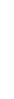
\includegraphics[max width=\linewidth, center]{external/whitespace-tikz/2cm.pdf}
\end{image}%
\item{}¿Cuántas patas tiene cada hormiga? Explica o muestra tu razonamiento.%
\begin{image}{0}{1}{0}{}%
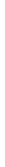
\includegraphics[max width=\linewidth, center]{external/whitespace-tikz/4cm.pdf}
\end{image}%
\end{enumerate}
%
\end{project}
\end{document}